\documentclass[../main.tex]{subfiles}

\usepackage{float} % Librería para presentación de imágenes

\begin{document}

En esta sección se va a describir como se van a integrar los datos en la aplicación. Se van a usar transformaciones XSLT, las cuales permiten definir plantillas para transformar un documento XML en otro tipo de documento (HTML en este caso) utilizando sintaxis XML.

\subsection{Transformación tabla bacterias}

En la interfaz de investigadores, para generar la tabla que aparece al pulsar en la bacteria se ha creado una transformación XSLT.

\hfill

Al principio de la transformación se ha creado una etiqueta \texttt{<style>} para poder dar formato a la tabla. A continuación, se ha creado la tabla y se han definido el nombre de las columnas. Para poder rellenar la tabla, dentro de cada fila (\textit{row}) del archivo XSL y se han seleccionado los nodos hijos mencionados anteriormente.

\hfill

En la imagen \ref{transB} se puede ver como se ha usado un \texttt{for-each} para ir recorriendo las filas cuyas bacterias tenga más de un 20\% de resistencia a los antibióticos. Después, se han ordenado las bacterias por mayor resistencia a antibióticos. Por último, se usa un \texttt{xsl:if} para comprobar que los datos no se repiten, pues hay varios estudios donde coinciden los resultados. Si la condición se cumple, se crea una nueva fila en la tabla con os datos seleccionados en los \texttt{xsl:value-of}.

\newpage

\begin{figure}[h]
    \centering
    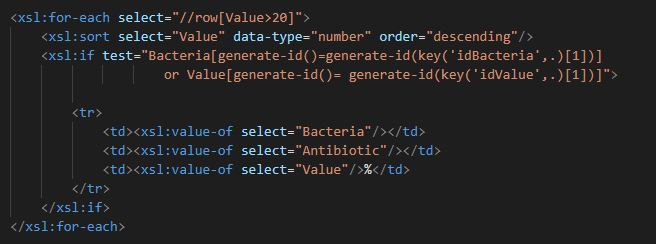
\includegraphics[scale=0.65]{images/trans_bacterias.JPG}
    \caption{Transformación tabla bacterias}
    \label{transB}
\end{figure}

\subsection{Transformación tabla grupos de estudio}

Se ha realizado otra transformación para el caso en el que el investigador pulse el botón de grupos de estudio. El principio es igual que en el caso anterior, se empieza dándole formato a la tabla y definiendo las columnas. En la imagen \ref{transG} se ve como se crean las columnas. Se vuelven a recorrer las distintas filas, esta vez sin condición, y se seleccionan los valores que necesitamos para rellenar la tabla.

\begin{figure}[h]
    \centering
    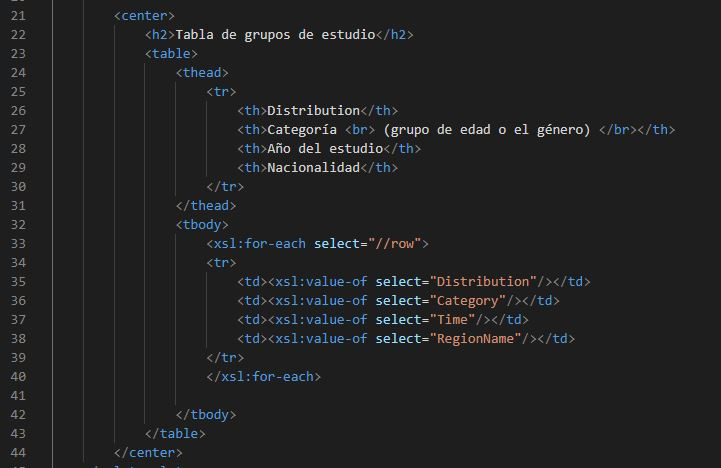
\includegraphics[scale=0.65]{images/trans_estudio.JPG}
    \caption{Transformación tabla grupos}
    \label{transG}
\end{figure}


\subsection{Transformaciones de las tablas del mapa}

Se ha realizado transformaciones para obtener información sobre aquellas bacterias con resistencia a antibióticos en ese país de Europa

\hfill

\begin{figure}[h]
    \centering
    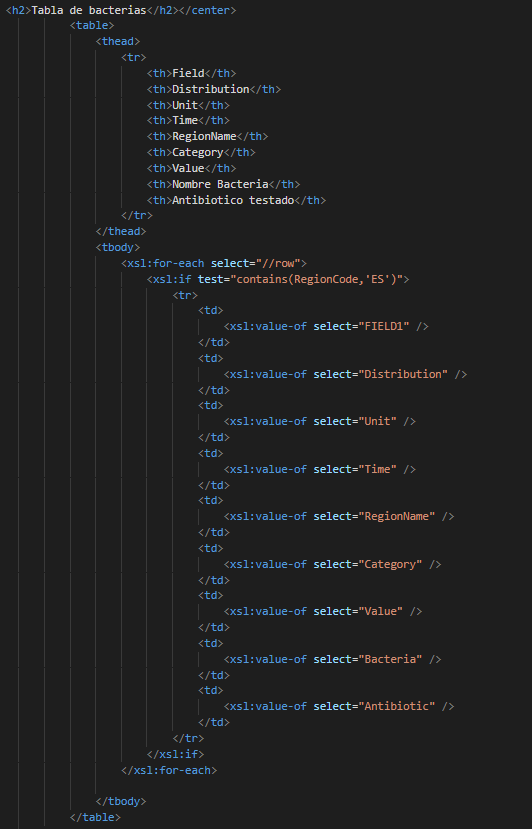
\includegraphics[scale=0.65]{images/trans_mapa.png}
    \caption{Transformación tabla grupos}
    \label{transMapa}
\end{figure}

\end{document}